\chapter{Generating random system properties}

One of the uses of random \gls{FOL} can be to generate random formula that represent system properties. That formula can be used as input for benchmark.

\section{Properties of computer systems}

System properties were first discussed in context of concurrency \cite{Lampert77} as a tool for formal verification multiprocess programs. One of first proposed properties were safety and liveness. These properties can apply to computer systems in general and be expressed in different formal systems.

\textbf{Liveness} \cite{Klimek99} is system property, that states, that something good will eventually happen.
Liveness formula guarantees that there is at least one case, where formula evaluates to true.

\textbf{Safety} \cite{Klimek99} is system property, that states, that something bad will never happens.
Safety formula must always be satisfied.

An informal example of system with liveness and safety properties could be an elevator. Statement: "Elevator will eventually stop" is liveness property of elevator as may be running now but eventually will hit the ceiling or floor. Statement: "Elevator must never run when the door is open" is safety property - the statement is always true.

\section{Properties of computer systems in first order logic}

In \gls{FOL} liveness and safety can be expressed as quantifiers, safety as universal quantifier and liveness as existential quantifier. 
If we were to use previously mentioned elevator example, the statements can be written as follows:

\begin{itemize}
  \item "Elevator will eventually stop" can be converted to logic formula: $\exists_t e(t)$ where predicate $e$ means "elevator is still", assuming $t<\infty$. The formula reads: there exists moment $t$ that the elevator is not moving
  \item "Elevator must never run when the door is open" can be converted to logic formula: $\forall_t \neg e(t) \land d(t)$ where predicate $e$ means "elevator is still" and $d$ means "doors are open". The formula reads: for every moment $t$ elevator is running and the doors are shut (at the same time).
\end{itemize}

\subsection{Properties of computer systems in first order logic in quantifier free}

Every \gls{FOL} can be converted to \gls{CNF}, so system properties can be also represented in \gls{CNF} but quantifiers must be also converted to CNF. The process of removing all the existential quantifiers from a formula is known as skolemization. The result is a formula in skolem normal form that is equivalent in computational complexity to the original. Skolemization follows several rules:


\begin{itemize}
  \item Variables bound by existential quantifiers which are not inside the scope of universal quantifiers can simply be replaced by constants - $\exists_t e(t)$ can be replaced by $e(f)$ where $f$ is new constant (functor)
  \item When the existential quantifier is inside a universal quantifier, the bound variable must be replaced by a Skolem function of the variables bound by universal quantifiers - $\forall_x  e(x) \land \exists_y e(t)$ can be replaced as $\forall_x e(x) \land e(f(x))$ 
\end{itemize}


Elevator example converted to quantifier free form looks as follows\footnote{removing quantifiers from first order logic can be automated with TPTP utility using TPTP2X utility, option \mintinline{text}{-t clausify:quaife}~\ref{sub:AdditionalToolsInTPTPLibrary} }::
\begin{itemize}
  \item "Elevator will eventually stop" $\exists_t e(t)$ in quantifier free form: $e(f)$ - new constant functor $f$ replaced variable $t$
  \item "Elevator must never run when the door is open" $\forall_t \neg e(t) \land d(t)$ in quantifier free form: $\neg e(X) \land d(Y)$ - 2 new variables $X$ and $Y$ replaced variable $t$ bounded to universal quantifier
\end{itemize}

In conclusion safety and liveness can be represented in CNF as 2 form of predicates: liveness as predicate, where arguments are only constant functors, safety as predicate where arguments are variables.

\section{Dataset with system properties}

The goal is to generate liveness and safety clauses, but do not mix them. In order to achieve that, class $PredicateGenerator$ needs to be modified to yield either formulas with all variables (safety) or formulas with 0-arity functor (liveness). To achieve that $PredicateGenerator$ was subclassed and used to create alternative version of $CNFFormulaGenerator$.

\begin{figure}[H]
\begin{centering}
  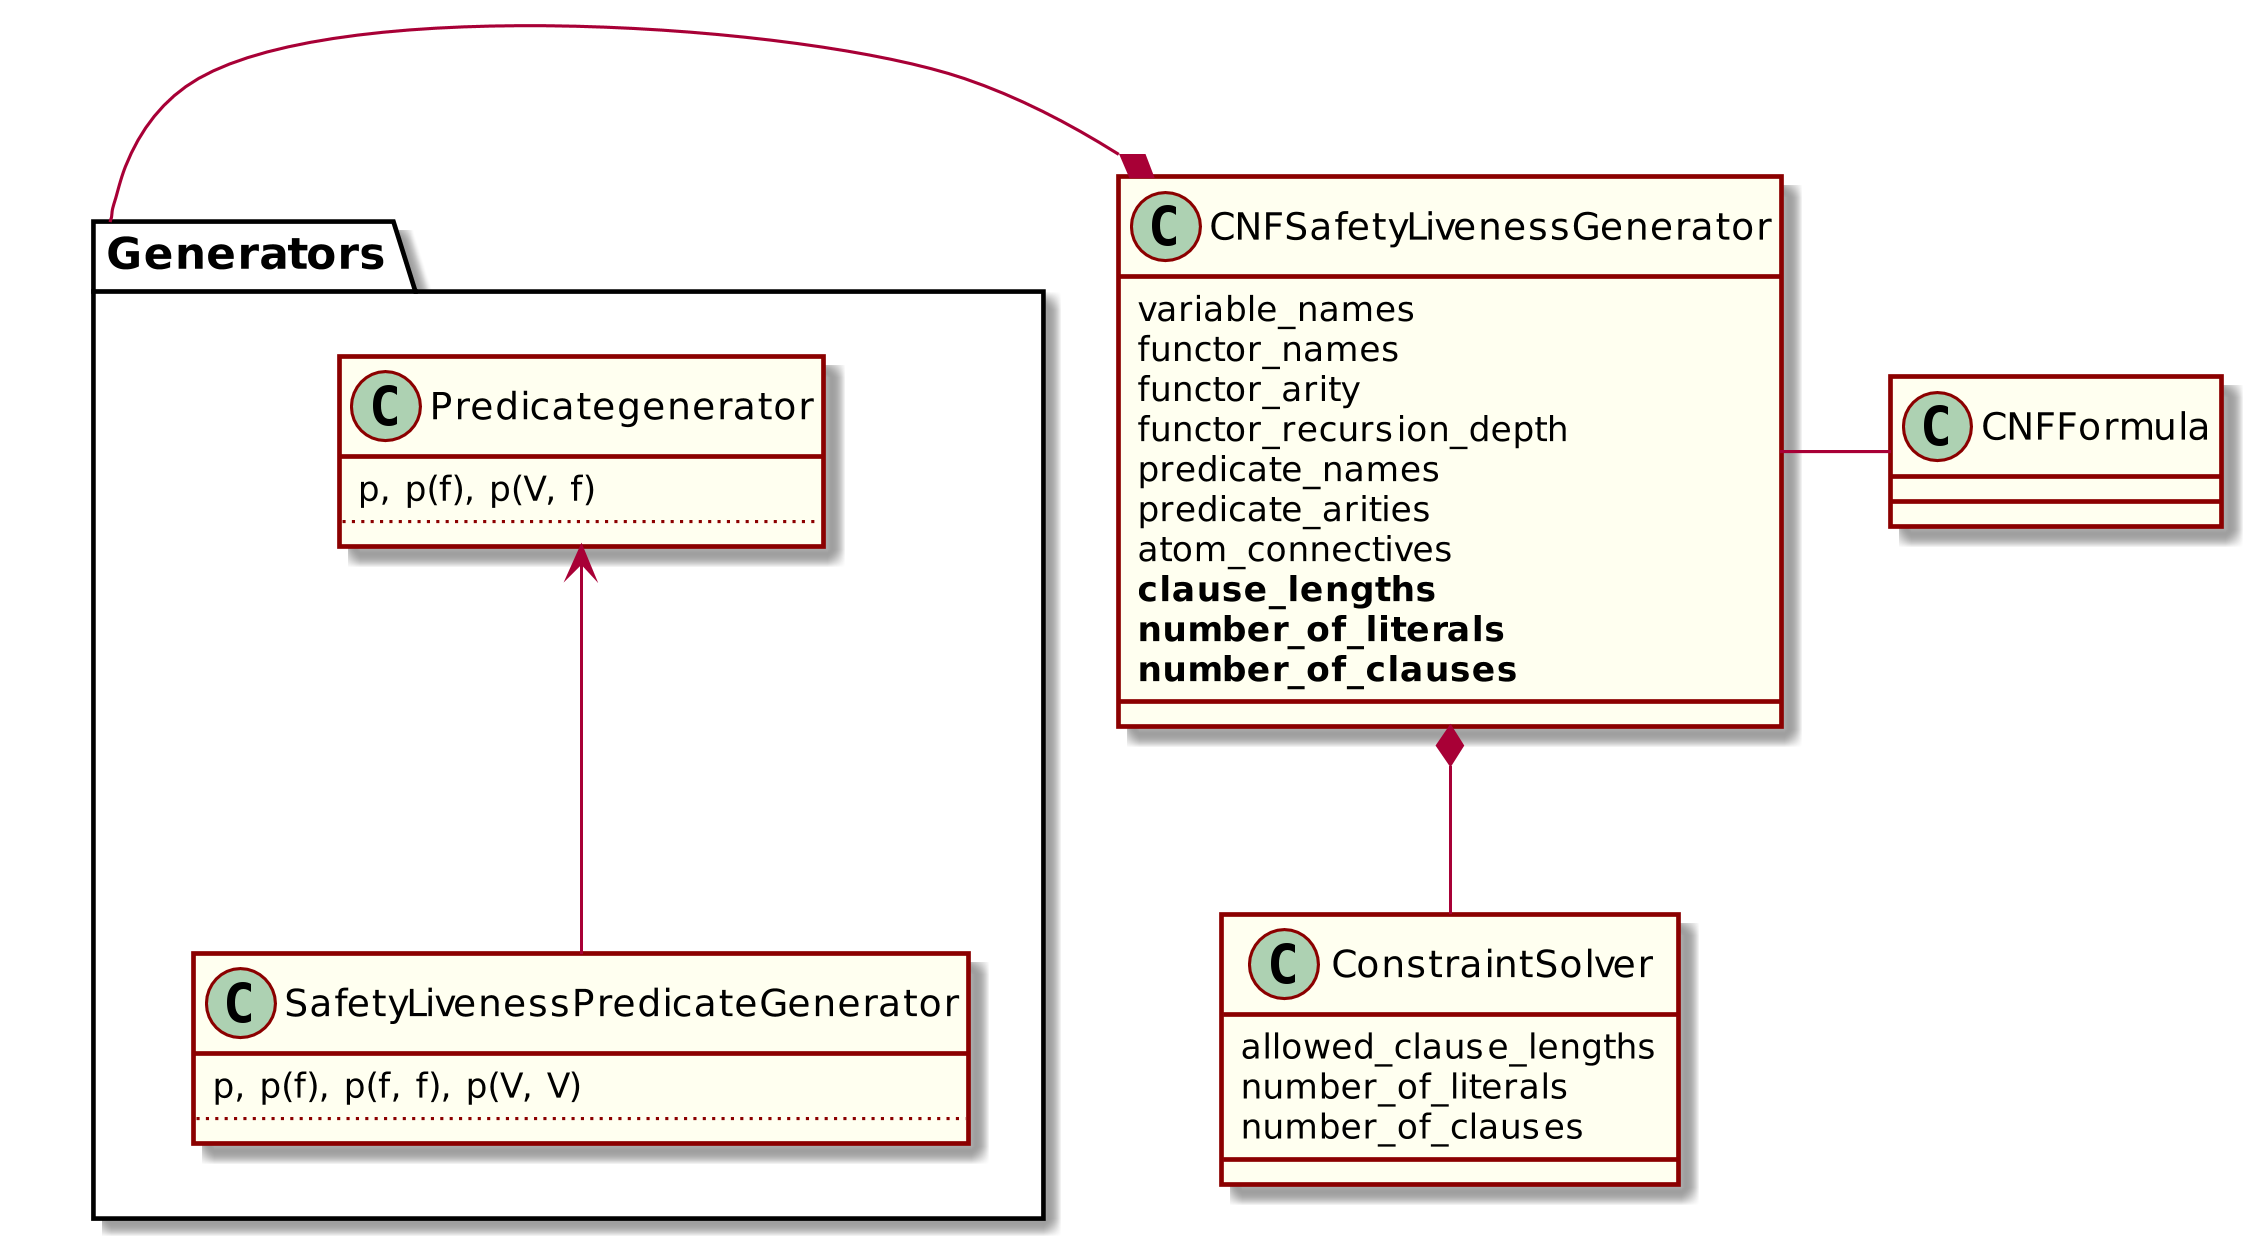
\includegraphics[width=\textwidth]{logic-formula-generator/fol/safety_liveness_predicate_generator.png}
  \caption{Subclassed PredicateGenerator mimics safety and liveness formulas}
\end{centering}
\end{figure}

In this study the impact of ratio of number of atoms to number of clauses will be presented.
Formulas with 1000 atoms and 100, 200, 300, 400, 500 clauses were generated, 50 for each combination, 250 in total. 50 formulas is rather small sample to reason about, but it was chosen because of time and hardware limitations. Number of atoms and number of clauses can vary within 5\%, although solver tends to yield small numbers first in general. The rest of parameters for formulas is shown in listing~\ref{lis:CNFSafetyLivenesSnippet}.

\subsection{Results}

Formulas were generated and were benchmarked against solvers Prover9 and SPASS. Results are shown in picture~\ref{pic:SPASSProverNumberOfClauses} and~\ref{pic:SPASSProverMemory}. Maximum execution time of single formula was trimmed at 300 seconds. 

First thing worth noting is SPASS solver is capable of solving much more formulas than Prover9. SPASS uses somewhat constant memory whereas Prover9 requires more memory the longer it runs.

It can be said that formulas with ratio atoms to clauses below 4 can be considered easy, as all of them were solved by both solvers.

\begin{listing}[ht]
  \caption{Snippet for generating dataset of safety and liveness formulas}
  \label{lis:CNFSafetyLivenesSnippet}
\begin{minted}{python}
gen = CNFSafetyLivenessGenerator(
    variable_names={f'V{i}' for i in range(10)},
    functor_names={f'f{i}' for i in range(20)}, functor_arity={0},
    functor_recursion_depth=0,
    predicate_names={f'p{i}' for i in range(20)}, predicate_arities={i for i in range(5)},
    atom_connectives={''},
    clause_lengths={i for i in range(2, 11)},
    number_of_clauses=IntegerRange.from_relative(number_of_clauses, threshold),
    number_of_literals=IntegerRange.from_relative(number_of_literals, threshold),
    literal_negation_chance=0.1,
)
\end{minted}
\end{listing}

\begin{listing}[H]
  \caption{Example of generated formula (limited)}
\begin{tptpcode}
% ----------------------------------------------------------------------------
% File      : 0.p 
% Syntax    : Number of clauses     :   95 ( 95 non-Horn;   0 unit;   - RR)
%             Number of atoms       :  950 (  0 equality)
%             Maximal clause size   :   10 ( 10 average)
%             Number of predicates  :   20 (206 propositional; 0-4 arity)
%             Number of functors    :   20 (940 constant;   0 arity)
%             Number of variables   :  943 (327 singleton)
%             Maximal term depth    :    0 (  - average)
% 
% ----------------------------------------------------------------------------
cnf(name,axiom,p4(V6)|p10(V1, V4, V9)|~p7|p17|p1(V4, V3, V9)|p7|p17|p1(f11, f11, f5)|p7|~p0(f2)).
cnf(name,axiom,p2(V7, V9)|p4(f19)|p2(f8, f5)|p10(f7, f8, f8)|p12|p6(V2, V6)|p14(f8, f16, f9, f16)|p3(f14, f3, f14, f18)|p11(V3, V9)|p12).
...
\end{tptpcode}
  \label{lis:TPTPExample}
\end{listing}

\newpage

\begin{figure}[H]
\centering
  \begin{subfigure}{0.8\textwidth}
\centering
  \includegraphics[width=\textwidth]{"logic-formula-generator/dataset_analysis/cnf charts/01 Prover9 number of clauses vs time".jpg}
  \label{pic:benchmark_results}
  \end{subfigure}

  \begin{subfigure}{\textwidth}
\centering
  \includegraphics[width=\textwidth]{"logic-formula-generator/dataset_analysis/cnf charts/11 SPASS number of clauses vs time".jpg}
  \end{subfigure}
  \caption{On left axis time of execution is presented (300s is max), marked with blue. On right axis ratio clauses to atoms is presented. Ratio 2 means there are 2 atoms for each clause}
  \label{pic:SPASSProverNumberOfClauses}
\end{figure}

\begin{figure}[H]
\centering
  \begin{subfigure}{0.8\textwidth}
\centering
  \includegraphics[width=\textwidth]{"logic-formula-generator/dataset_analysis/cnf charts/02 Prover9 number of clauses vs peak memory".jpg}
  \label{pic:benchmark_results}
  \end{subfigure}

  \begin{subfigure}{\textwidth}
\centering
\includegraphics[width=\textwidth]{"logic-formula-generator/dataset_analysis/cnf charts/12 SPASS number of clauses vs peak memory".jpg}
  \end{subfigure}
  \caption{On left axis peak RAM memory is presented, marked with blue. On right axis ratio clauses to atoms is presented. Ratio 2 means there are 2 atoms for each clause}
  \label{pic:SPASSProverMemory}
\end{figure}

% \section{Modified dataset}
%
% TODO
%
% \begin{figure}[H]
% \begin{centering}
%   \includegraphics[width=\textwidth]{"logic-formula-generator/fol/safety_liveness_predicate_generator_1_in_10".png}
%   \caption{Subclassed PredicateGenerator mimics safety and liveness formulas}
% \end{centering}
% \end{figure}
%
% \subsection{Results}
%
% TODO
%
% Charts are only placeholders:

% \newpage
%
% \begin{figure}[H]
% \centering
%   \begin{subfigure}{0.8\textwidth}
% \centering
%   \includegraphics[width=\textwidth]{"logic-formula-generator/dataset_analysis/cnf charts/01 Prover9 number of clauses vs time".jpg}
%   % \label{pic:}
%   \end{subfigure}
%
%   \begin{subfigure}{\textwidth}
% \centering
%   \includegraphics[width=\textwidth]{"logic-formula-generator/dataset_analysis/cnf charts/11 SPASS number of clauses vs time".jpg}
%   \end{subfigure}
%   \caption{On left axis time of execution is presented (300s is max), marked with blue. On right axis ratio clauses to atoms is presented. Ratio 2 means there are 2 atoms for each clause}
%   % \label{pic:}
% \end{figure}
%
% \begin{figure}[H]
% \centering
%   \begin{subfigure}{0.8\textwidth}
% \centering
%   \includegraphics[width=\textwidth]{"logic-formula-generator/dataset_analysis/cnf charts/02 Prover9 number of clauses vs peak memory".jpg}
%   % \label{pic:}
%   \end{subfigure}
%
%   \begin{subfigure}{\textwidth}
% \centering
% \includegraphics[width=\textwidth]{"logic-formula-generator/dataset_analysis/cnf charts/12 SPASS number of clauses vs peak memory".jpg}
%   \end{subfigure}
%   \caption{On left axis peak RAM memory is presented, marked with blue. On right axis ratio clauses to atoms is presented. Ratio 2 means there are 2 atoms for each clause}
%   % \label{pic:}
% \end{figure}
%
